\frame{
  \frametitle{Introduction}

  \begin{itemize}
    \item Billiard ball bouncing in a square
    \item Assume no gravity or friction
    \item Examine sequence of side collisions
  \end{itemize}
}

\subsection{Examples}

\frame{
  \frametitle{Example}

  \begin{example}
    Examine the periodic sequence: `abab`
  \end{example}

  \begin{figure}
    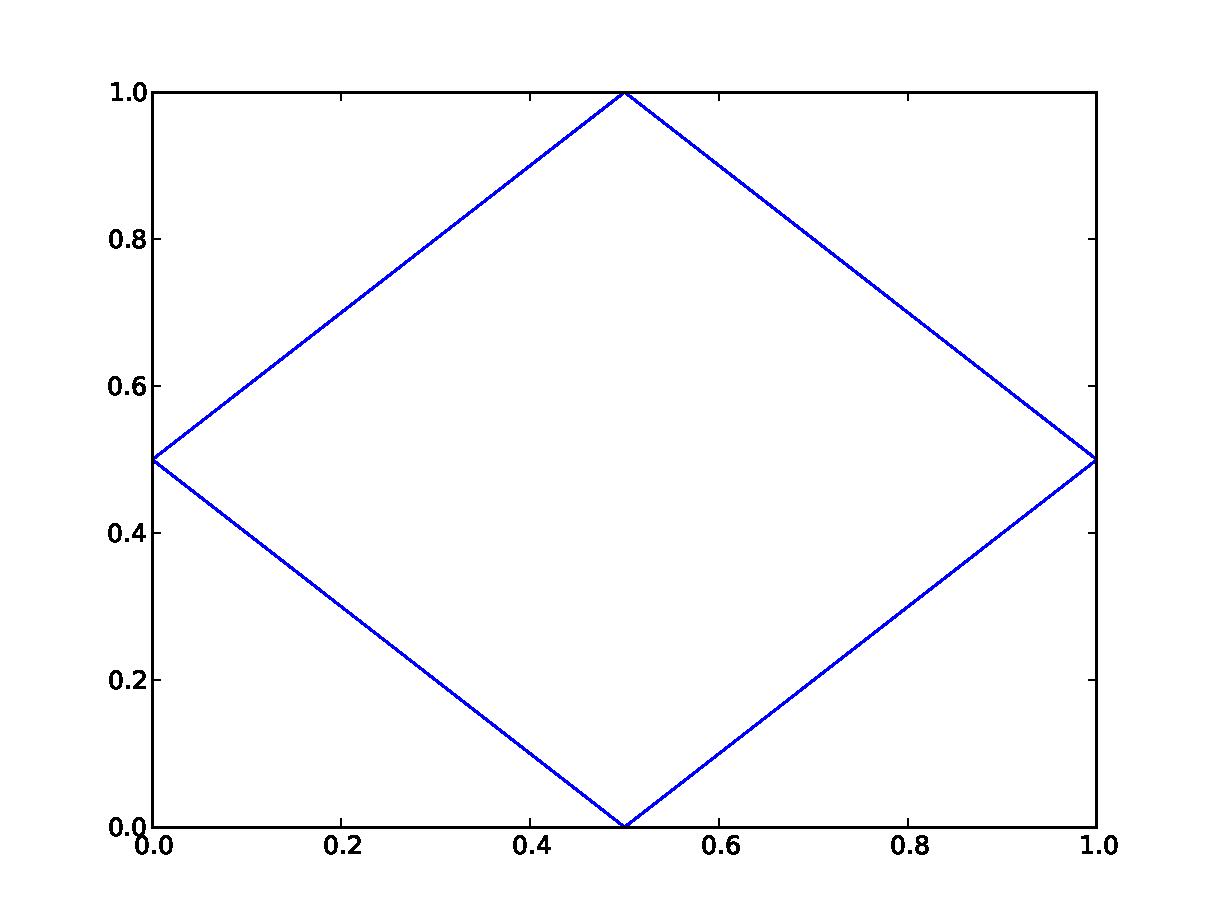
\includegraphics[width=3in]{abab.pdf}
  \end{figure}
}

\frame{
  \frametitle{Another Example}

  \begin{example}
    Examine the periodic sequence: `aaabaaab`
  \end{example}

  \begin{figure}
    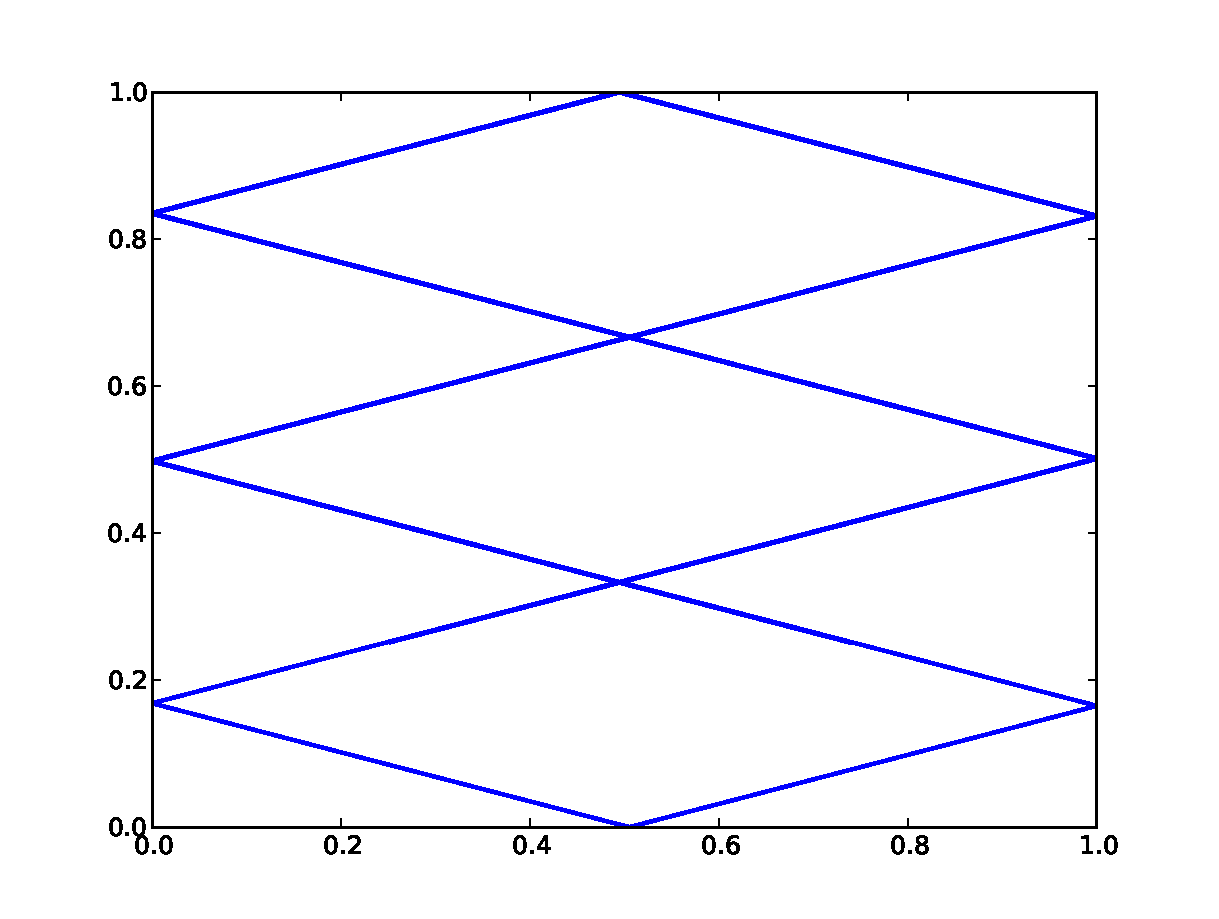
\includegraphics[width=3in]{aaabaaab.pdf}
  \end{figure}
}

\subsection{Outline}

\frame{
  \frametitle{Presentation Outline}
  \tableofcontents
}

\subsection{Notation and Problem Statement}

\frame{
  \frametitle{Notation}
  \begin{definition}
    A table $T \in \R^2$ is the unit square. Opposite sides of the table are labeled $a$ and $b$.
  \end{definition}

  \begin{figure}
    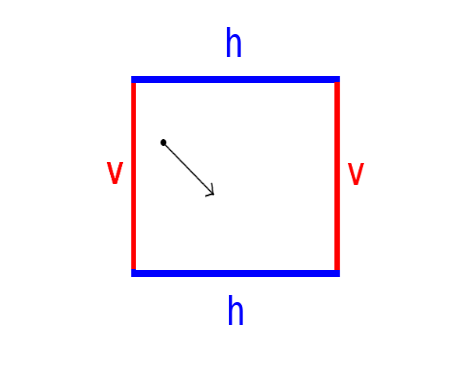
\includegraphics[width=2in]{square_with_sides.png}
  \end{figure}
}

\frame{
  \frametitle{Notation}

  \begin{definition}
     A ball $p \in T$ begins at position $\vec{r}_0 \in T$ with initial velocity $\vec{v}_0 \ne 0$. When the ball collides with an edge of the table, it reflects such that the component of its velocity normal to the edge is negated after the collision, and its component tangent to the edge is unchanged.
  \end{definition}

  \begin{figure}
    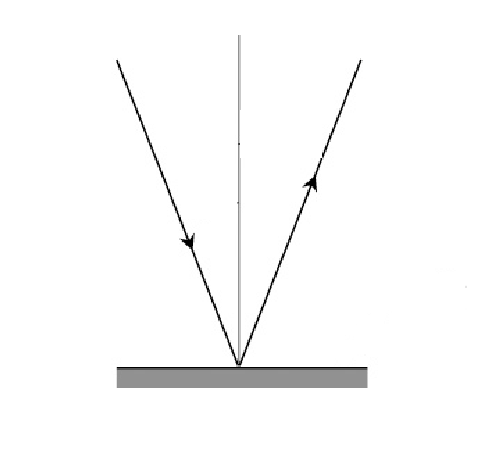
\includegraphics[height=1.5in]{particle_collision.png}
  \end{figure}
}

\frame{
  \frametitle{Notation}
  \begin{definition}
    \textbf{Collision string:} list of the sides of the table that a ball collides with, ordered by collision time. e.g. `abaaabaaaab'.

    \textbf{Primary side}: side appearing most often in a collision string.

    \textbf{Secondary side} the other side.
  \end{definition}

  \pause

  \begin{definition}
    \textbf{Primary substring:} a subsequence from the collision string which contains the primary side collisions that occur between consecutive secondary side collisions.
  \end{definition}

  \pause

  \begin{example}
    \textbf{Collision string}: `aabaaabaabaaab`, \textbf{Primary substrings}: `aa`, `aaa`
  \end{example}
}

\frame{
  \frametitle{Problem Statement}

  Problem: Characterize the properties of collision sequences.

  \begin{itemize}
    \item Given a sequence of $a$'s and $b$'s, determine if it is a valid collision sequence.
    \item Given a valid collision sequence, determine a possible starting position and velocity.
  \end{itemize}
}

